\documentclass[pdftex,12pt,letter]{article}
\usepackage[binary-units=true]{siunitx}
\usepackage[margin=0.75in]{geometry}
\usepackage{verbatim}
\usepackage{graphicx}
\usepackage{cite}
\usepackage{color}
\usepackage[pdftex,pdfpagelabels,bookmarks,hyperindex,hyperfigures]{hyperref}
\usepackage{xspace}
%\usepackage[firstpage]{draftwatermark}


\bibliographystyle{unsrt}

\newcommand{\fixme}[1]{\textbf{FIXME: #1}}    
\newcommand{\pd}{ProtoDUNE\xspace}

\title{Online Systems for the Single-Phase \pd}
\date{\today}
\author{M.Potekhin, B. Viren}

\begin{document}
%\SetWatermarkText{DRAFT}
%\SetWatermarkLightness{0.9}
%\SetWatermarkScale{3}

\maketitle

\begin{abstract}
\noindent This document has been prepared to inform the DUNE Technical Board about the current status
(as of June 2016) and direction of R\&D in the area of the Single-Phase \pd DAQ interface to online/offline data storage
and raw data handling. It does not cover internal architecture of the various DAQ components but is focused on
issues of interfaces, throughput and online storage requirements and design, as well as some aspects of prompt
processing of the data.
\end{abstract}

\tableofcontents

\pagebreak

\section{Overview}

This purpose of this document is to provide a concise summary of
the R\&D, status report and plans related to the elements of the DAQ which interface
the online buffer, design of that buffer and strategy and tools
for data transport to mass storage and transfer from CERN to remote Grid sites.
The document is based on the materials being prepared for the \pd Technical Design Report  (work in progress)
and on documents and plans developed earlier, in particular DocDB 1209 and \textit{Design of
the Data Management System for the protoDUNE Experiment} (DocDB 1212).

Data rate and volume will be the defining factor for the design choice and scale of \pd online and other computing systems.
%Depending on the plan of measurements for \pd
%(in development at the time of writing), beam characteristics that will be realized
%anda few other parameters precise estimates of data rates and volume aren't available just yet.
At present, preliminary estimates are available for a few realistic scenarios. As the R\&D is progressing, this will
be used to firm up the requirements, and finally the system configuration, scale and performance.

The overall design for the protoDUNE computing can be described as consisting of the following major components:
\begin{itemize}

\item The online data storage and management system which interfaces the DAQ and which is tasked with buffering
the data and transporing it to mass storage at CERN and beyond.

\item The offline system for data distribution and processing on the Grid (e.g. calibration, production and reconstruction). A special case
of such processing is the so-called \textit{prompt processing}, which aims to perform partial reconstruction of the data for QA/QC purposes
with a short turnaround time and can be considered a more advanced type of monitoring. The prompt processing system
does have an important interface to the online systems by virtue of sharing the same central staging area in CERN EOS.

\item A Metadata and file catalog system -- crucial for operation of both components listed above.

\end{itemize}

\noindent In the following we describe the requirements, preliminary design options and some anticipated parameters
of these components.

\section{The Storage Buffer}
\subsection{Factors Impacting the Design of the Buffer}
The storage buffer is the primary system to which the DAQ will write its data.
According to CERN rules and common practices, this buffer is essentialy local to the experiment
(in contrast to the CERN campus where the central storage facilities are located) and is
required to potentially cache as much as
three days worth of nominal data acquisition. One of the motivations is to ensure
the ability of the experiment to run even with some network disruptions in the CERN area.
During nominal running the buffer serves as a staging area for data transfer
to CERN EOS disk system and effectively reduces coupling between various components of the
data transfer system.

According to the current plan, this transfer shall be performed by
an instance of the Fermilab File Transfer System (called F-FTS or simply `` FTS'') deployed
at the experiment.

The expected data rates exceed the capabilities of commodity hardware
unless a parallel architecture is implemented. One of the possibilities is to
exploit the parallelism already present in the DAQ itself, however this
would lead to a tighter coupling between the DAQ and its buffer system and
may require a more careful design and integration testing as compared to a more
losely organized system.

More than one approach is being considered as there are a few crucial
requirements to be finalized which will have strong impact on the design.
and which can be satisfied in more than one way. For example, some of such
requirements are:

\begin{itemize}

\item having sequential trigger numbers (or event numbers) in any given raw data file

\item contiguous readout fragments for a given trigger in a raw data file

\item redundancy of the storage system and possible failover/recovery mode

\item maximum latency of the data transport to EOS and other mass storage at CERN and FNAL

\end{itemize}

\noindent Also open at this point is the question of whether some of these capabilities (such as ordering of data elements
inside a file) can be ``outsourced'' from the online to offline processing.

In the following sections, a review of our current understanding of
the SP data rates is given, then the DAQ is described at a high level.
Finally, a number of optional designs for a unified online/offline
buffer are described.

\subsection{Data Rates}

The ``\pd/SP Data Scenarios'' spreadsheet~\cite{data-scenarios}
describes three possible running conditions and estimates for their
resulting data volumes and rates and interpretations in terms of
network and disk bandwidth.  It also includes estimates for non-beam
trigger for acquiring additional cosmic-$\mu$ data.  Some highlights
of these estimates for the mid-range (so called ``Central'')
scenario are in Table~\ref{tab:central}.

\begin{table}[htbp]
  \centering
  \begin{tabular}[h]{l|r}
    Trigger rate & \SI{25}{\Hz} \\
    Spill time & \SI{4.5}{\second} \\
    Cycle time & \SI{22.5}{\second} \\
    Readout time & \SI{5}{\milli\second} \\
    \#APA & 6 \\
    \hline
    Readout & \SI{230}{\mega\byte} \\
    Lossless Compression & $\times$4 \\
    Instant rate & \SI{1440}{\mega\byte\per\second} \\
    Average rate & \SI{288}{\mega\byte\per\second} \\
    \hline
    3-Day volume & \SI{75}{\tera\byte} \\
    Total volume of data for the run & \SI{1.5}{\peta\byte} \\
    \hline\hline
    cosmic-$\mu$ & $\times$2 \\
  \end{tabular}
  \caption{Parameters characterizing the ``Central'' data taking scenario.}
  \label{tab:central}
\end{table}


\noindent Based on preliminary plan for calibrations which involves measuring a few types of cosmic $\mu$ tracks
(e.g. at different angles, stopped vs not stopped etc),
the current assumption is that for every beam trigger one non-beam
trigger be acquired out-of-spill. 
This assumption represents a doubling of the data rates and volumes presented in Table~\ref{tab:central}.
The instant and average rates are those for when the beam is spilling or if the rate is amortized over the
entire beam cycle. With the  numbers presented above some level of parallelism
is needed to sustain the expected bandwidth on commodity hardware,
conservatively defined as Gbps network interfaces and \SI{50}{\mega\byte\per\second} disk I/O. 
%The second issue is that the scenario is based on uncertain parameters
%which are known to lead to underestimates.  The scenario is expected
%to grow substantially as they are better known.  In particular:

%\begin{itemize}
%\item A \SI{25}{\Hz} trigger rate is assumed although the beam can   deliver hundreds of \si{\Hz} of particles.  
% \item Trigger efficiency and purity is assumed to be 100\% meaning  exactly 5M triggers are needed to satisfy the run plan.
%\item It is assumed the SP detector will achieve a noise level no   worse than MicroBooNE and thus can also achieve the associated  compression factor of $\times5$.
%\end{itemize}

It is useful to consider cases which can lead to more demanding conditions than listed in Table\,\ref{tab:central},
such as:
\begin{itemize}

\item The trigger rate goes to \SI{50}{\Hz} in order to ``catch up'' with the run plan after some delays

\item The triggering ends up being only 50\% pure requiring acquisition of more triggers (e.g. in excess of the planned 25M)

\item The noise level achieved is closer to that of the 35t causing   compression factor to fall to $\times 2$.

\end{itemize}

%If all these extreme contingencies were to occur together their affect
%on the buffer is estimated as in Table~\ref{tab:expansion}.
%\begin{table}[htbp]
% \centering
%  \begin{tabular}[h]{r|rl}
%   volume & $\times10$ & \SI{3.3}{\peta\byte} total raw data \\
%  \hline
%  writes & $\times25$ & 13 Gbps, 65 parallel HDDs, \\
%  \hline
% buffer & $\times25$ & \SI{850}{\tera\byte}, 3-days\\
%  \end{tabular}
%  \caption{Worse case scenarios where trigger rate, trigger selection and noise are such that they all increase the amount of data.}
%  \label{tab:expansion}
%\end{table}

\noindent If these factors were all to materialize together, they represent a range of scale
of more than an order of magnitude. While such dramatic shift in requirements is not expected,
it is necessary to design systems with reliable scaling behavior in order to have headroom
to ensure a useful sample of data can be collected by SP-\pd.


%  We must plan to implement a system
%that is adequate for the ``worse reasonable case'' as the actual data
%rates will not be known until SP begins commissioning.  Such concrete
%planning and procurement must follow.  For this document we limit the
%discussion to just the design.

\section{DAQ Throughput and Multiplicity}

This section describes the basic elements of DAQ and how it is modeled in order to understand
its throughput and the node multiplicity.  The basic DAQ up to event
building is described and the model is applied to the nominal data
scenario.
\subsection{DAQ Model}
The connectivity of a portion of the upstream part of the DAQ is
illustrated in a general way in Fig.~\ref{fig:upstream}.
\begin{figure}[htbp]
  \centering
  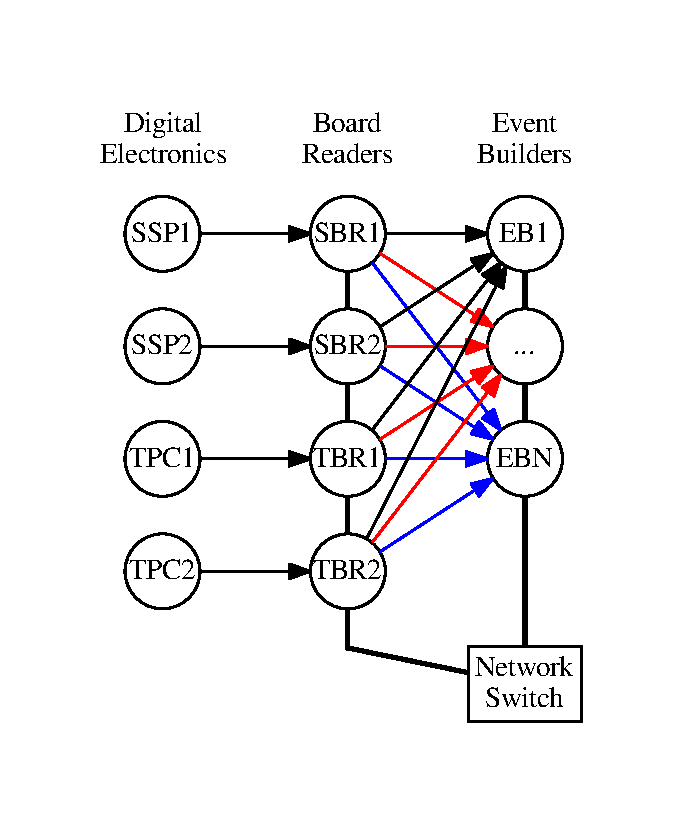
\includegraphics[width=0.5\textwidth]{upstream.pdf}
  \caption{Some fraction of the upstream portion of the DAQ.}
  \label{fig:upstream}
\end{figure}
A node in
the Digital Electronics (DE) layer provides the source of data for one
portion of the detector, either optical (SSP) or wire waveforms (TPC).
These fragments enter the DAQ via Board Readers (BR).  Each fragment
from a common trigger carries a common trigger number which is
indicated in the diagram by a colored arrow.  Based on that number,
fragments from the same trigger are sent to a common event builder
(EB) node for assembly.  In the figure, all fragments from a ``black
trigger'' is sent to EB1 and all fragments from a
``\textcolor{blue}{blue trigger}'' are sent to EBN.

The number of nodes in the BR layer is determined by channel
multiplicity of the detector electronics that are to be read out.
Given the nature of the DAQ application, there is freedom to choose
the multiplicities of the Event Builder and subsequent layers.  The optimum choice is a balance of performance (more
nodes) and cost (fewer nodes).  For a given set of assumptions a
number of minimum requirements can be derived.

Work is currently under way to develop quantitative models of possible
network configurations such as depicted in Fig.~\ref{fig:upstream},
and to perform requisite optimization.


\section{DAQ Storage Options}

Starting at the EB layer of Fig.~\ref{fig:upstream} a number of
options are considered that extend the distributed DAQ to meet the
buffer while not creating a bottleneck.  They differ in trade offs of
node multiplicity and features.

\subsection{Immediate Write}

The simplest extension of the basic upstream DAQ configuration is to
add local disks and an instance of F-FTS to the computers hosting the
EB services.  This option is termed \textit{Immediate Write} and the salient
parts are illustrated for a single host in Fig.~\ref{fig:immediate}.

\begin{figure}[htbp]
  \centering
  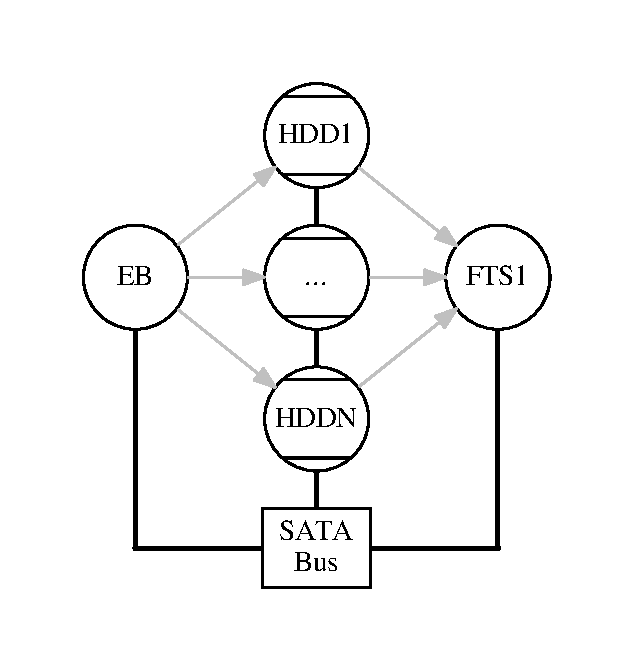
\includegraphics[width=10cm]{eb2ld.pdf}
  \caption{The \textit{Immediate Write} option to connect one EB to local
    buffer disk storage.}
  \label{fig:immediate}
\end{figure}

In this local context of a single host the same basic model can be
applied.  The ``nodes'' here include a process that writes the data to
a storage unit (HDD) and then makes this data available to F-FTS,
which also fits in to the model as a node. While this design is simple and requires only minimal extra hardware
it has the following consequences:  

\begin{itemize}

\item Interlaced triggers.  The events from the EB node that are saved
  to disk will not be sequential because the EB does not receive
  sequential triggers from the upstream BRs.

\item Tight coupling.  The EB processing and FTS-related processing
  (metadata and checksumming) may lead to CPU contention.
\end{itemize}

\subsection{Sorted}

Having events in data file in a perfectly serial (sorted) order is not a firm requirement at this point.
However, such option is still being considered. It requires an extra layer of \textit{Event Sorter} (ES) nodes.  These nodes must maintain
a buffer in memory of some number of events which can be as many as
what an entire file holds.  However, this load can be spread across
multiple ES nodes so that multiple events in multiple files need not
be cached in a single memory system.  As detailed next, the resulting
files will themselves still be interlaced but this out-of-order issue
is erased through the use of a file catalog.

\subsection{Decoupled Write}

This variant extends \textit{Immediate Write} to move the EB (or ES)
node off of the same host as the storage.  This requires a new service
to accept data from the EB (or ES) node and write it to disk.  This
new service can be based on artDAQ which makes it part of the DAQ
proper.  Alternatively, it can use another protocol such as XRootD in
which case the EB (or ES) must be developed to speak this protocol.
If additional processing is required (such as metadata file production
and checksumming) as the data is written then an artDAQ implementation
for this node is likely best.

\subsection{Preprocessed}

If the requirement of sequential triggers is necessary then it can be
accomplished in an offline context.  The essential idea is that an
offline process close to the source of the interlaced data files reads
in multiple stream, performs deinterlacing and writes out sequential
files.  This will be a highly I/O bound and data intensive job.

\section{Software Provisioning for Online Systems}
As mentioned above, the role of the online buffer is to give the experiment the capacity
to run relatively autonomously, e.g. if the network connection to the main CERN campus
goes down for a period of time. For the same reason, the online systems including the
DAQ, online monitoring and elements of the data transfer system need to be able to operate
using locally installed software. This therefore is among the design provisions.


\section{From Online to Offline}

\subsection{Raw Data Flow in \pd}
\label{sec:raw_concept}
%%%%%%%%%%%%%%%%%%%%%%%%
\begin{figure}[tbh]
\centering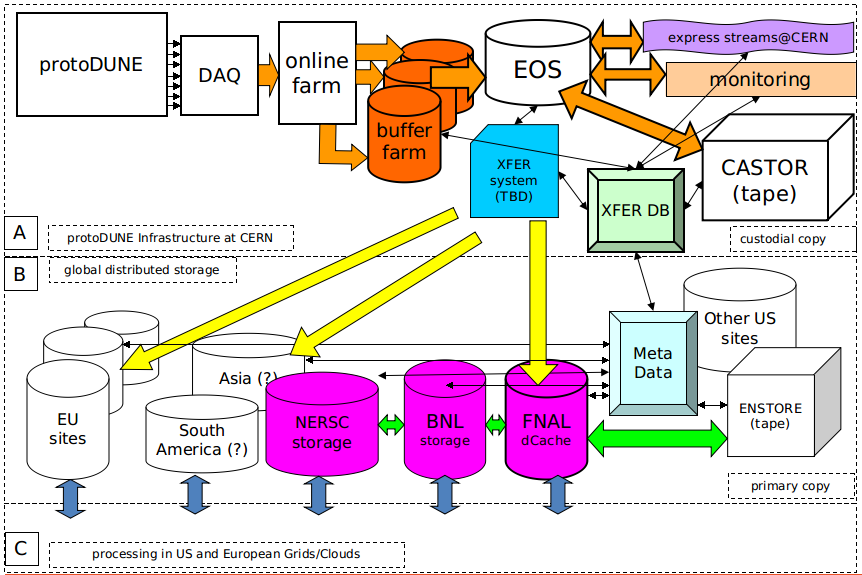
\includegraphics[width=\linewidth]{protoDUNE_raw_data_concept.png}
\caption{\label{fig:raw_concept}Conceptual diagram of the flow of raw data in \pd}
\end{figure}
%%%%%%%%%%%%%%%%%%%%%%%%

\noindent
Conceptual diagram of the raw data flow in \pd is presented in Fig.\ref{fig:raw_concept}. It shows the general logic
of data flow, and does not include specific assumptions about what system will be used to actually move the data.
It also reflects the central role of CERN EOS in the \pd raw data management scheme. This is motivated by the experience
and architecture of the LHC experiments.

EOS serves as the staging area from which the data gets committed to CASTOR
and from which it is transmitted to a number of endpoints including principal data centers such as FNAL and others.
It is also used to provide input to QA and other express processing streams at CERN (sec.\,\ref{sec:prompt_processing}).

Data centers at BNL and NERSC are placed in this diagram for illustration purposes. Any other institution possessing adequate
resources can participate in this data distriburtion scheme if desired. According to the design presented in DUNE DocDB~1212
this part of the data transmission process is also handled by an instance of F-FTS.


\subsection{Prompt Processing}
\label{sec:prompt_processing}
In the present context, \textit{Prompt Processing} means a number of fast signal processing and reconstruction processes
(also called ``express stream'' sometimes) which process a fraction of raw data. Its main purpose is to aid in QA of the data
and produce quick calibrations which may be necessary for high quality monitoring of the detector. As one example,
calculating frequency spectra of noise and watching its level, evolution and other characteristincs is an important aspect of ensuring
the stability of the readout chain.

It is understood
that a limited number of metrics will be calculated to make the proccess as quick as possible in order to enable
the operators to take action should the QA process indicate a potential problem in the detector or the data.
The following parameters of prompt processing need to considered:
\begin{itemize}
\item Desired turnaround time.
\item Location of the computing resources utilized.
\item Fraction and type of data to be processed in this manner.
\end{itemize}

\noindent As to the latter item, it is estimated that processing roughly 1\% of the data stream collected by the detector will
be enough to meet most important goals of prompt processing. 
The general strategy is to locate a significant fraction of the prompt processing capability at CERN, at a scale adequate for the mid-range
data taking scenario such as presented in Table\, \ref{tab:central}. A very preliminary estimate indicated that about 750 cores
will be needed to cope with processing at that rate.

If placement of these resources at CERN is problematic and/or it becomes necessary to scale up from
this capacity due to a decision to increase the trigger rate,
the plan is to take advantage of the high bandwidth of the network connection between
CERN and a few significant sites in the US (such as FNAL, BNL and others) and do additional processing there.

Managing the ``prompt processing'' streams is a subset of the wider issue of workload management, and outside of
the scope of this document. It's worth noting however that a capable WMS with ability to distribute amd shift the
workload between CERN and other Grid sites as necessary may prove essential for efficient operation of \pd.

\section{Summary}
 A few possible architectures of the online storage have been identified.
Work is under way to create a framework (e.g. discrete-event simulation) needed to evaluate possible storage architectures
with regard to bandwidth and potential bottlenecks, as well as most cost-effective configuration.
Anticipated progress on the measurements plan (formulated by the respective WG) will allow
to firm up the numbers and finalize the proposed hardware and middleware configurations.

Preliminary scope of prompt processing (express streams) has been identified along with a rough estimate of the needed
computing resources.

\bibliography{citedb}

\end{document}

%%% Local Variables:
%%% mode: latex
%%% TeX-master: t
%%% End:
